\documentclass[11pt,compress,t,notes=noshow, xcolor=table]{beamer}
%<<setup-child, include = FALSE>>=
%library(knitr)
%library(qrmix)
%library(mlr)
%library(quantreg)
%library(reshape2)
%set_parent("../style/preamble.Rnw")
%@

% graphicx and color are loaded via lmu-lecture.sty
% maxwidth is the original width if it is less than linewidth
% otherwise use linewidth (to make sure the graphics do not exceed the margin)
% TODO: Remove once cleared to be superfluous
% \makeatletter
% \def\maxwidth{ %
%   \ifdim\Gin@nat@width>\linewidth
%     \linewidth
%   \else
%     \Gin@nat@width
%   \fi
% }
% \makeatother

% ---------------------------------%
% latex-math dependencies, do not remove:
% - mathtools
% - bm
% - siunitx
% - dsfont
% - xspace
% ---------------------------------%

%--------------------------------------------------------%
%       Language, encoding, typography
%--------------------------------------------------------%

\usepackage[english]{babel}
\usepackage[utf8]{inputenc} % Enables inputting UTF-8 symbols
% Standard AMS suite (loaded via lmu-lecture.sty)

% Font for double-stroke / blackboard letters for sets of numbers (N, R, ...)
% Distribution name is "doublestroke"
% According to https://mirror.physik.tu-berlin.de/pub/CTAN/fonts/doublestroke/dsdoc.pdf
% the "bbm" package does a similar thing and may be superfluous.
% Required for latex-math
\usepackage{dsfont}

% bbm – "Blackboard-style" cm fonts (https://www.ctan.org/pkg/bbm)
% Used to be in common.tex, loaded directly after this file
% Maybe superfluous given dsfont is loaded
% TODO: Check if really unused?
% \usepackage{bbm}

% bm – Access bold symbols in maths mode - https://ctan.org/pkg/bm
% Required for latex-math, preferred over \boldsymbol
% https://tex.stackexchange.com/questions/3238/bm-package-versus-boldsymbol
\usepackage{bm}

% pifont – Access to PostScript standard Symbol and Dingbats fonts
% Used for \newcommand{\xmark}{\ding{55}, which is never used
% aside from lecture_advml/attic/xx-automl/slides.Rnw
% \usepackage{pifont}

% Quotes (inline and display), provdes \enquote
% https://ctan.org/pkg/csquotes
\usepackage{csquotes}

% Adds arg to enumerate env, technically superseded by enumitem according
% to https://ctan.org/pkg/enumerate
% Replace with https://ctan.org/pkg/enumitem ?
% Even better: enumitem is not really compatible with beamer and breaks all sorts of things
% particularly the enumerate environment. The enumerate package also just isn't required
% from what I can tell so... don't re-add it I guess?
% \usepackage{enumerate}

% Line spacing - provides \singlespacing \doublespacing \onehalfspacing
% https://ctan.org/pkg/setspace
% \usepackage{setspace}

% mathtools – Mathematical tools to use with amsmath
% https://ctan.org/pkg/mathtools?lang=en
% latex-math dependency according to latex-math repo
\usepackage{mathtools}

% Maybe not great to use this https://tex.stackexchange.com/a/197/19093
% Use align instead -- TODO: Global search & replace to check, eqnarray is used a lot
% $ rg -f -u "\begin{eqnarray" -l | grep -v attic | awk -F '/' '{print $1}' | sort | uniq -c
%   13 lecture_advml
%   14 lecture_i2ml
%    2 lecture_iml
%   27 lecture_optimization
%   45 lecture_sl
\usepackage{eqnarray}
% For shaded regions / boxes
% Used sometimes in optim
% https://www.ctan.org/pkg/framed
\usepackage{framed}

%--------------------------------------------------------%
%       Cite button (version 2024-05)
%--------------------------------------------------------%

% Superseded by style/ref-buttons.sty, kept just in case these don't work out somehow.

% Note this requires biber to be in $PATH when running,
% telltale error in log would be e.g. Package biblatex Info: ... file 'authoryear.dbx' not found
% aside from obvious "biber: command not found" or similar.
% Tried moving this to lmu-lecture.sty but had issues I didn't quite understood,
% so it's here for now.

\usepackage{hyperref}

% Only try adding a references file if it exists, otherwise
% this would compile error when references.bib is not found
% NOTE: Bibliography packages (usebib, biblatex) are now loaded by ref-buttons.sty when needed
% This keeps all bibliography-related setup in one place

% Legacy \citelink command removed - superseded by ref-buttons.sty

%--------------------------------------------------------%
%       Displaying code and algorithms
%--------------------------------------------------------%

% Reimplements verbatim environments: https://ctan.org/pkg/verbatim
% verbatim used sed at least once in
% supervised-classification/slides-classification-tasks.tex
% Removed since code should not be put on slides anyway
% \usepackage{verbatim}

% Both used together for algorithm typesetting, see also overleaf: https://www.overleaf.com/learn/latex/Algorithms
% algorithmic env is also used, but part of the bundle:
%   "algpseudocode is part of the algorithmicx bundle, it gives you an improved version of algorithmic besides providing some other features"
% According to https://tex.stackexchange.com/questions/229355/algorithm-algorithmic-algorithmicx-algorithm2e-algpseudocode-confused
\usepackage{algorithm}
\usepackage{algpseudocode}

%--------------------------------------------------------%
%       Tables
%--------------------------------------------------------%

% multi-row table cells: https://www.namsu.de/Extra/pakete/Multirow.html
% Provides \multirow
% Used e.g. in evaluation/slides-evaluation-measures-classification.tex
\usepackage{multirow}

% colortbl: https://ctan.org/pkg/colortbl
% "The package allows rows and columns to be coloured, and even individual cells." well.
% Provides \columncolor and \rowcolor
% \rowcolor is used multiple times, e.g. in knn/slides-knn.tex
\usepackage{colortbl}

% long/multi-page tables: https://texdoc.org/serve/longtable.pdf/0
% Not used in slides
% \usepackage{longtable}

% pretty table env: https://ctan.org/pkg/booktabs
% Is used
% Defines \toprule
\usepackage{booktabs}

%--------------------------------------------------------%
%       Figures: Creating, placing, verbing
%--------------------------------------------------------%

% wrapfig - Wrapping text around figures https://de.overleaf.com/learn/latex/Wrapping_text_around_figures
% Provides wrapfigure environment -used in lecture_optimization
\usepackage{wrapfig}

% Sub figures in figures and tables
% https://ctan.org/pkg/subfig -- supersedes subfigure package
% Provides \subfigure
% \subfigure not used in slides but slides-tuning-practical.pdf errors without this pkg, error due to \captionsetup undefined
\usepackage{subfig}

% Actually it's pronounced PGF https://en.wikibooks.org/wiki/LaTeX/PGF/TikZ
\usepackage{tikz}

% No idea what/why these settings are what they are but I assume they're there on purpose
\usetikzlibrary{shapes,arrows,automata,positioning,calc,chains,trees, shadows}
\tikzset{
  %Define standard arrow tip
  >=stealth',
  %Define style for boxes
  punkt/.style={
    rectangle,
    rounded corners,
    draw=black, very thick,
    text width=6.5em,
    minimum height=2em,
    text centered},
  % Define arrow style
  pil/.style={
    ->,
    thick,
    shorten <=2pt,
    shorten >=2pt,}
}

%--------------------------------------------------------%
%       Beamer setup and custom macros & environments
%--------------------------------------------------------%

% Main sty file for beamer setup (layout, style, lecture page numbering, etc.)
% For long-term maintenance, this may me refactored into a more modular set of .sty files
\usepackage{../../style/lmu-lecture}
% Custom itemize wrappers, itemizeS, itemizeL, etc
\usepackage{../../style/customitemize}
% Custom framei environment, uses custom itemize!
\usepackage{../../style/framei}
% Custom frame2 environment, allows specifying font size for all content
\usepackage{../../style/frame2}
% Column layout macros
\usepackage{../../style/splitV}
% \image and derivatives
\usepackage{../../style/image}
% New generation of reference button macros
\usepackage{../../style/ref-buttons}

% Used regularly
\let\code=\texttt

% Not sure what/why this does
\setkeys{Gin}{width=0.9\textwidth}

% -- knitr leftovers --
% These may be used by knitr/R Markdown workflows in other lectures
\makeatletter
\def\maxwidth{ %
  \ifdim\Gin@nat@width>\linewidth
    \linewidth
  \else
    \Gin@nat@width
  \fi
}
\makeatother

% Define colors for syntax highlighting (may be used by knitr)
\definecolor{fgcolor}{rgb}{0.345, 0.345, 0.345}
\definecolor{shadecolor}{rgb}{.97, .97, .97}

% knitr code output environment
\newenvironment{knitrout}{}{}


% Can't find a reason why common.tex is not just part of this file?
\input{../../style/common}

\input{../../latex-math/basic-math}
% machine learning
\newcommand{\Xspace}{\mathcal{X}} % X, input space
\newcommand{\Yspace}{\mathcal{Y}} % Y, output space
\newcommand{\Zspace}{\mathcal{Z}} % Z, space of sampled datapoints
\newcommand{\nset}{\{1, \ldots, n\}} % set from 1 to n
\newcommand{\pset}{\{1, \ldots, p\}} % set from 1 to p
\newcommand{\gset}{\{1, \ldots, g\}} % set from 1 to g
\newcommand{\Pxy}{\mathbb{P}_{xy}} % P_xy
\newcommand{\Exy}{\mathbb{E}_{xy}} % E_xy: Expectation over random variables xy
\newcommand{\xv}{\mathbf{x}} % vector x (bold)
\newcommand{\xtil}{\tilde{\mathbf{x}}} % vector x-tilde (bold)
\newcommand{\yv}{\mathbf{y}} % vector y (bold)
\newcommand{\xy}{(\xv, y)} % observation (x, y)
\newcommand{\xvec}{\left(x_1, \ldots, x_p\right)^\top} % (x1, ..., xp)
\newcommand{\Xmat}{\mathbf{X}} % Design matrix
\newcommand{\allDatasets}{\mathds{D}} % The set of all datasets
\newcommand{\allDatasetsn}{\mathds{D}_n}  % The set of all datasets of size n
\newcommand{\D}{\mathcal{D}} % D, data
\newcommand{\Dn}{\D_n} % D_n, data of size n
\newcommand{\Dtrain}{\mathcal{D}_{\text{train}}} % D_train, training set
\newcommand{\Dtest}{\mathcal{D}_{\text{test}}} % D_test, test set
\newcommand{\xyi}[1][i]{\left(\xv^{(#1)}, y^{(#1)}\right)} % (x^i, y^i), i-th observation
\newcommand{\Dset}{\left( \xyi[1], \ldots, \xyi[n]\right)} % {(x1,y1)), ..., (xn,yn)}, data
\newcommand{\defAllDatasetsn}{(\Xspace \times \Yspace)^n} % Def. of the set of all datasets of size n
\newcommand{\defAllDatasets}{\bigcup_{n \in \N}(\Xspace \times \Yspace)^n} % Def. of the set of all datasets
\newcommand{\xdat}{\left\{ \xv^{(1)}, \ldots, \xv^{(n)}\right\}} % {x1, ..., xn}, input data
\newcommand{\ydat}{\left\{ \yv^{(1)}, \ldots, \yv^{(n)}\right\}} % {y1, ..., yn}, input data
\newcommand{\yvec}{\left(y^{(1)}, \hdots, y^{(n)}\right)^\top} % (y1, ..., yn), vector of outcomes
\newcommand{\greekxi}{\xi} % Greek letter xi
\renewcommand{\xi}[1][i]{\xv^{(#1)}} % x^i, i-th observed value of x
\newcommand{\yi}[1][i]{y^{(#1)}} % y^i, i-th observed value of y
\newcommand{\xivec}{\left(x^{(i)}_1, \ldots, x^{(i)}_p\right)^\top} % (x1^i, ..., xp^i), i-th observation vector
\newcommand{\xj}{\xv_j} % x_j, j-th feature
\newcommand{\xjvec}{\left(x^{(1)}_j, \ldots, x^{(n)}_j\right)^\top} % (x^1_j, ..., x^n_j), j-th feature vector
\newcommand{\phiv}{\mathbf{\phi}} % Basis transformation function phi
\newcommand{\phixi}{\mathbf{\phi}^{(i)}} % Basis transformation of xi: phi^i := phi(xi)

%%%%%% ml - models general
\newcommand{\lamv}{\bm{\lambda}} % lambda vector, hyperconfiguration vector
\newcommand{\Lam}{\Lambda}	 % Lambda, space of all hpos
% Inducer / Inducing algorithm
\newcommand{\preimageInducer}{\left(\defAllDatasets\right)\times\Lam} % Set of all datasets times the hyperparameter space
\newcommand{\preimageInducerShort}{\allDatasets\times\Lam} % Set of all datasets times the hyperparameter space
% Inducer / Inducing algorithm
\newcommand{\ind}{\mathcal{I}} % Inducer, inducing algorithm, learning algorithm

% continuous prediction function f
\newcommand{\ftrue}{f_{\text{true}}}  % True underlying function (if a statistical model is assumed)
\newcommand{\ftruex}{\ftrue(\xv)} % True underlying function (if a statistical model is assumed)
\newcommand{\fx}{f(\xv)} % f(x), continuous prediction function
\newcommand{\fdomains}{f: \Xspace \rightarrow \R^g} % f with domain and co-domain
\newcommand{\Hspace}{\mathcal{H}} % hypothesis space where f is from
\newcommand{\Hall}{\mathcal{H}_{\text{all}}} % unrestricted hypothesis space
\newcommand{\fbayes}{f^{\ast}} % Bayes-optimal model
\newcommand{\fxbayes}{f^{\ast}(\xv)} % Bayes-optimal model
\newcommand{\fkx}[1][k]{f_{#1}(\xv)} % f_j(x), discriminant component function
\newcommand{\fhspace}{\hat f_{\Hspace}} % fhat_H
\newcommand{\fh}{\hat{f}} % f hat, estimated prediction function
\newcommand{\fxh}{\fh(\xv)} % fhat(x)
\newcommand{\fxt}{f(\xv ~|~ \thetav)} % f(x | theta)
\newcommand{\fxi}{f\left(\xv^{(i)}\right)} % f(x^(i))
\newcommand{\fxih}{\hat{f}\left(\xv^{(i)}\right)} % f(x^(i))
\newcommand{\fxit}{f\big(\xv^{(i)} ~|~ \thetav\big)} % f(x^(i) | theta)
\newcommand{\fhD}{\fh_{\D}} % fhat_D, estimate of f based on D
\newcommand{\fhDtrain}{\fh_{\Dtrain}} % fhat_Dtrain, estimate of f based on D
\newcommand{\fhDnlam}{\fh_{\Dn, \lamv}} %model learned on Dn with hp lambda
\newcommand{\fhDlam}{\fh_{\D, \lamv}} %model learned on D with hp lambda
\newcommand{\fhDnlams}{\fh_{\Dn, \lamv^\ast}} %model learned on Dn with optimal hp lambda
\newcommand{\fhDlams}{\fh_{\D, \lamv^\ast}} %model learned on D with optimal hp lambda

% discrete prediction function h
\newcommand{\hx}{h(\xv)} % h(x), discrete prediction function
\newcommand{\hh}{\hat{h}} % h hat
\newcommand{\hxh}{\hat{h}(\xv)} % hhat(x)
\newcommand{\hxt}{h(\xv | \thetav)} % h(x | theta)
\newcommand{\hxi}{h\left(\xi\right)} % h(x^(i))
\newcommand{\hxit}{h\left(\xi ~|~ \thetav\right)} % h(x^(i) | theta)
\newcommand{\hbayes}{h^{\ast}} % Bayes-optimal classification model
\newcommand{\hxbayes}{h^{\ast}(\xv)} % Bayes-optimal classification model

% yhat
\newcommand{\yh}{\hat{y}} % yhat for prediction of target
\newcommand{\yih}{\hat{y}^{(i)}} % yhat^(i) for prediction of ith targiet
\newcommand{\resi}{\yi- \yih}

% theta
\newcommand{\thetah}{\hat{\theta}} % theta hat
\newcommand{\thetav}{\bm{\theta}} % theta vector
\newcommand{\thetavh}{\bm{\hat\theta}} % theta vector hat
\newcommand{\thetat}[1][t]{\thetav^{[#1]}} % theta^[t] in optimization
\newcommand{\thetatn}[1][t]{\thetav^{[#1 +1]}} % theta^[t+1] in optimization
\newcommand{\thetahDnlam}{\thetavh_{\Dn, \lamv}} %theta learned on Dn with hp lambda
\newcommand{\thetahDlam}{\thetavh_{\D, \lamv}} %theta learned on D with hp lambda
\newcommand{\mint}{\min_{\thetav \in \Theta}} % min problem theta
\newcommand{\argmint}{\argmin_{\thetav \in \Theta}} % argmin theta

% densities + probabilities
% pdf of x
\newcommand{\pdf}{p} % p
\newcommand{\pdfx}{p(\xv)} % p(x)
\newcommand{\pixt}{\pi(\xv~|~ \thetav)} % pi(x|theta), pdf of x given theta
\newcommand{\pixit}[1][i]{\pi\left(\xi[#1] ~|~ \thetav\right)} % pi(x^i|theta), pdf of x given theta
\newcommand{\pixii}[1][i]{\pi\left(\xi[#1]\right)} % pi(x^i), pdf of i-th x

% pdf of (x, y)
\newcommand{\pdfxy}{p(\xv,y)} % p(x, y)
\newcommand{\pdfxyt}{p(\xv, y ~|~ \thetav)} % p(x, y | theta)
\newcommand{\pdfxyit}{p\left(\xi, \yi ~|~ \thetav\right)} % p(x^(i), y^(i) | theta)

% pdf of x given y
\newcommand{\pdfxyk}[1][k]{p(\xv | y= #1)} % p(x | y = k)
\newcommand{\lpdfxyk}[1][k]{\log p(\xv | y= #1)} % log p(x | y = k)
\newcommand{\pdfxiyk}[1][k]{p\left(\xi | y= #1 \right)} % p(x^i | y = k)

% prior probabilities
\newcommand{\pik}[1][k]{\pi_{#1}} % pi_k, prior
\newcommand{\pih}{\hat{\pi}} % pi hat, estimated prior (binary classification)
\newcommand{\pikh}[1][k]{\hat{\pi}_{#1}} % pi_k hat, estimated prior
\newcommand{\lpik}[1][k]{\log \pi_{#1}} % log pi_k, log of the prior
\newcommand{\pit}{\pi(\thetav)} % Prior probability of parameter theta

% posterior probabilities
\newcommand{\post}{\P(y = 1 ~|~ \xv)} % P(y = 1 | x), post. prob for y=1
\newcommand{\postk}[1][k]{\P(y = #1 ~|~ \xv)} % P(y = k | y), post. prob for y=k
\newcommand{\pidomains}{\pi: \Xspace \rightarrow \unitint} % pi with domain and co-domain
\newcommand{\pibayes}{\pi^{\ast}} % Bayes-optimal classification model
\newcommand{\pixbayes}{\pi^{\ast}(\xv)} % Bayes-optimal classification model
\newcommand{\piastxtil}{\pi^{\ast}(\xtil)} % Bayes-optimal classification model
\newcommand{\piastkxtil}{\pi^{\ast}_k(\xtil)} % Bayes-optimal classification model for k-th class
\newcommand{\pix}{\pi(\xv)} % pi(x), P(y = 1 | x)
\newcommand{\piv}{\bm{\pi}} % pi, bold, as vector
\newcommand{\pikx}[1][k]{\pi_{#1}(\xv)} % pi_k(x), P(y = k | x)
\newcommand{\pikxt}[1][k]{\pi_{#1}(\xv ~|~ \thetav)} % pi_k(x | theta), P(y = k | x, theta)
\newcommand{\pixh}{\hat \pi(\xv)} % pi(x) hat, P(y = 1 | x) hat
\newcommand{\pikxh}[1][k]{\hat \pi_{#1}(\xv)} % pi_k(x) hat, P(y = k | x) hat
\newcommand{\pixih}{\hat \pi(\xi)} % pi(x^(i)) with hat
\newcommand{\pikxih}[1][k]{\hat \pi_{#1}(\xi)} % pi_k(x^(i)) with hat
\newcommand{\pdfygxt}{p(y ~|~\xv, \thetav)} % p(y | x, theta)
\newcommand{\pdfyigxit}{p\left(\yi ~|~\xi, \thetav\right)} % p(y^i |x^i, theta)
\newcommand{\lpdfygxt}{\log \pdfygxt } % log p(y | x, theta)
\newcommand{\lpdfyigxit}{\log \pdfyigxit} % log p(y^i |x^i, theta)

% probabilistic
\newcommand{\bayesrulek}[1][k]{\frac{\P(\xv | y= #1) \P(y= #1)}{\P(\xv)}} % Bayes rule
\newcommand{\muv}{\bm{\mu}} % expectation vector of Gaussian
\newcommand{\muk}[1][k]{\bm{\mu_{#1}}} % mean vector of class-k Gaussian (discr analysis)
\newcommand{\mukh}[1][k]{\bm{\hat{\mu}_{#1}}} % estimated mean vector of class-k Gaussian (discr analysis)

% residual and margin
\newcommand{\rx}{r(\xv)} % residual 
\newcommand{\eps}{\epsilon} % residual, stochastic
\newcommand{\epsv}{\bm{\epsilon}} % residual, stochastic, as vector
\newcommand{\epsi}{\epsilon^{(i)}} % epsilon^i, residual, stochastic
\newcommand{\epsh}{\hat{\epsilon}} % residual, estimated
\newcommand{\epsvh}{\hat{\epsv}} % residual, estimated, vector
\newcommand{\yf}{y \fx} % y f(x), margin
\newcommand{\yfi}{\yi \fxi} % y^i f(x^i), margin
\newcommand{\Sigmah}{\hat \Sigma} % estimated covariance matrix
\newcommand{\Sigmahj}{\hat \Sigma_j} % estimated covariance matrix for the j-th class
\newcommand{\nux}{\nu(\xv)} % nu(x) = y * f(x)

% ml - loss, risk, likelihood
\newcommand{\Lyf}{L\left(y, f\right)} % L(y, f), loss function
% \newcommand{\Lypi}{L\left(y, \pi\right)} % L(y, pi), loss function
\newcommand{\Lxy}{L\left(y, \fx\right)} % L(y, f(x)), loss function
\newcommand{\Lxyi}{L\left(\yi, \fxi\right)} % loss of observation
\newcommand{\Lxyt}{L\left(y, \fxt\right)} % loss with f parameterized
\newcommand{\Lxyit}{L\left(\yi, \fxit\right)} % loss of observation with f parameterized
\newcommand{\Lxym}{L\left(\yi, f\left(\bm{\tilde{x}}^{(i)} ~|~ \thetav\right)\right)} % loss of observation with f parameterized
\newcommand{\Lpixy}{L\left(y, \pix\right)} % loss in classification
% \newcommand{\Lpiy}{L\left(y, \pi\right)} % loss in classification
\newcommand{\Lpiv}{L\left(y, \piv\right)} % loss in classification
\newcommand{\Lpixyi}{L\left(\yi, \pixii\right)} % loss of observation in classification
\newcommand{\Lpixyt}{L\left(y, \pixt\right)} % loss with pi parameterized
\newcommand{\Lpixyit}{L\left(\yi, \pixit\right)} % loss of observation with pi parameterized
% \newcommand{\Lhy}{L\left(y, h\right)} % L(y, h), loss function on discrete classes
\newcommand{\Lhxy}{L\left(y, \hx\right)} % L(y, h(x)), loss function on discrete classes
\newcommand{\Lr}{L\left(r\right)} % L(r), loss defined on residual (reg) / margin (classif)
\newcommand{\lone}{|y - \fx|} % L1 loss
\newcommand{\ltwo}{\left(y - \fx\right)^2} % L2 loss
\newcommand{\lbernoullimp}{\ln(1 + \exp(-y \cdot \fx))} % Bernoulli loss for -1, +1 encoding
\newcommand{\lbernoullizo}{- y \cdot \fx + \log(1 + \exp(\fx))} % Bernoulli loss for 0, 1 encoding
\newcommand{\lcrossent}{- y \log \left(\pix\right) - (1 - y) \log \left(1 - \pix\right)} % cross-entropy loss
\newcommand{\lbrier}{\left(\pix - y \right)^2} % Brier score
\newcommand{\risk}{\mathcal{R}} % R, risk
\newcommand{\riskbayes}{\mathcal{R}^\ast}
\newcommand{\riskf}{\risk(f)} % R(f), risk
\newcommand{\riskdef}{\E_{y|\xv}\left(\Lxy \right)} % risk def (expected loss)
\newcommand{\riskt}{\mathcal{R}(\thetav)} % R(theta), risk
\newcommand{\riske}{\mathcal{R}_{\text{emp}}} % R_emp, empirical risk w/o factor 1 / n
\newcommand{\riskeb}{\bar{\mathcal{R}}_{\text{emp}}} % R_emp, empirical risk w/ factor 1 / n
\newcommand{\riskef}{\riske(f)} % R_emp(f)
\newcommand{\risket}{\mathcal{R}_{\text{emp}}(\thetav)} % R_emp(theta)
\newcommand{\riskr}{\mathcal{R}_{\text{reg}}} % R_reg, regularized risk
\newcommand{\riskrt}{\mathcal{R}_{\text{reg}}(\thetav)} % R_reg(theta)
\newcommand{\riskrf}{\riskr(f)} % R_reg(f)
\newcommand{\riskrth}{\hat{\mathcal{R}}_{\text{reg}}(\thetav)} % hat R_reg(theta)
\newcommand{\risketh}{\hat{\mathcal{R}}_{\text{emp}}(\thetav)} % hat R_emp(theta)
\newcommand{\LL}{\mathcal{L}} % L, likelihood
\newcommand{\LLt}{\mathcal{L}(\thetav)} % L(theta), likelihood
\newcommand{\LLtx}{\mathcal{L}(\thetav | \xv)} % L(theta|x), likelihood
\newcommand{\logl}{\ell} % l, log-likelihood
\newcommand{\loglt}{\logl(\thetav)} % l(theta), log-likelihood
\newcommand{\logltx}{\logl(\thetav | \xv)} % l(theta|x), log-likelihood
\newcommand{\errtrain}{\text{err}_{\text{train}}} % training error
\newcommand{\errtest}{\text{err}_{\text{test}}} % test error
\newcommand{\errexp}{\overline{\text{err}_{\text{test}}}} % avg training error

% lm
\newcommand{\thx}{\thetav^\top \xv} % linear model
\newcommand{\olsest}{(\Xmat^\top \Xmat)^{-1} \Xmat^\top \yv} % OLS estimator in LM

\input{../../latex-math/ml-eval}
\input{../../latex-math/ml-trees} % For the comparison of Brier and Gini index

\title{Introduction to Machine Learning}

\begin{document}
    
\titlemeta{% Chunk title (example: CART, Forests, Boosting, ...), can be empty
    Advanced Risk Minimization
  }{% Lecture title  
    Bernoulli Loss
  }{% Relative path to title page image: Can be empty but must not start with slides/
  figure/plot_bernoulli_prob.png
  }{
  \item Know the Bernoulli loss and related losses (log-loss, logistic loss, Binomial loss)
  \item Derive the risk minimizer
  \item Derive the optimal constant model 
  \item Understand the connection between log-loss and entropy splitting 
}

\begin{vbframe}{Bernoulli Loss}

\vspace*{-0.5cm}
\begin{eqnarray*}
  L(y, \fx) &=& \log(1+\exp(-y \cdot \fx)) \quad \text{for } y \in \setmp\\
  L(y, \fx) &=& - y \cdot \fx + \log(1 + \exp(\fx)) \quad \text{for } y \in \setzo 
\end{eqnarray*}

\begin{itemize}
  % \item Two equivalent formulations: labels $y \in \setmp$ or $y \in \setzo$
  \item Two equivalent formulations for different label encodings
  \item Negative log-likelihood of Bernoulli model, e.g., logistic regression
  \item Convex, differentiable
  %\item Pseudo-residuals (0/1 case): $\tilde{r} = y - \frac{1}{1+\exp(-\fx)}$\\   
  % Interpretation: $L1$ distance between 0/1-labels and posterior prob!
\end{itemize}

\vspace{0.2cm}
\begin{center}
% \includegraphics[width = 9cm ]{figure_man/bernoulli.png} \\
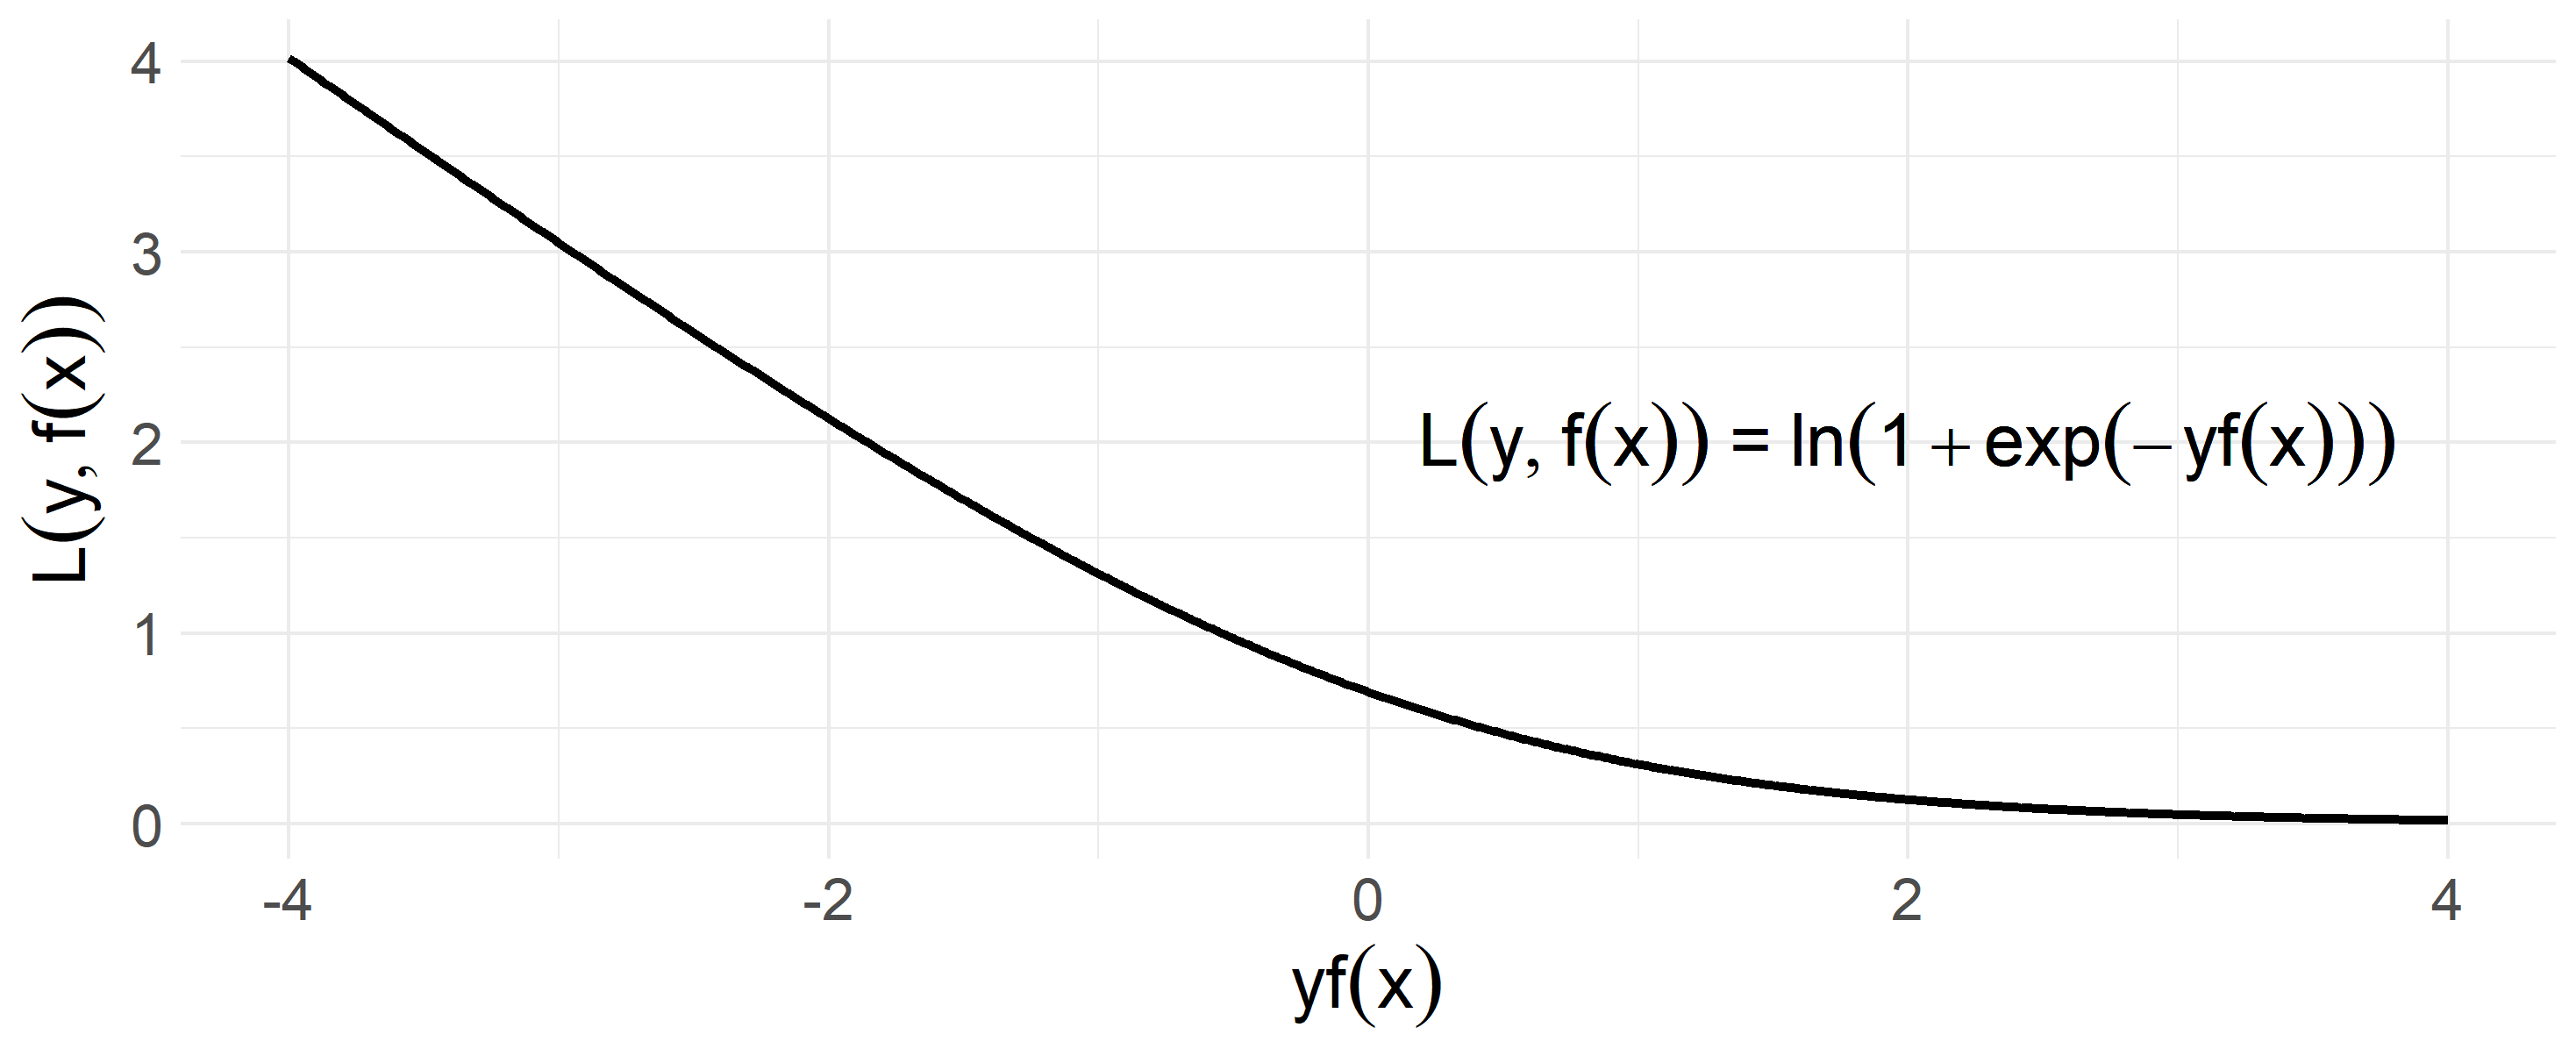
\includegraphics[width = 8cm ]{figure/plot_bernoulli_plusmin_encoding.png}
\end{center}

\end{vbframe}




\begin{vbframe}{Bernoulli loss on probabilities}

If scores are transformed into probabilities by the logistic function  $\pix = \left(1 + \exp(- \fx)\right)^{-1}$ (or equivalently if $f(x) = \log\left(\frac{\pix}{1 - \pix}\right)$ are the log-odds of $\pix$), we arrive at another equivalent formulation of the loss, where $y$ is again encoded as $\setzo$:

  $$
    L(y, \pix) = - y \log \left(\pix\right) - (1 - y) \log \left(1 - \pix\right). 
  $$
  
\begin{center}
% \includegraphics[width = 10cm ]{figure_man/bernoulli-loss.png} \\
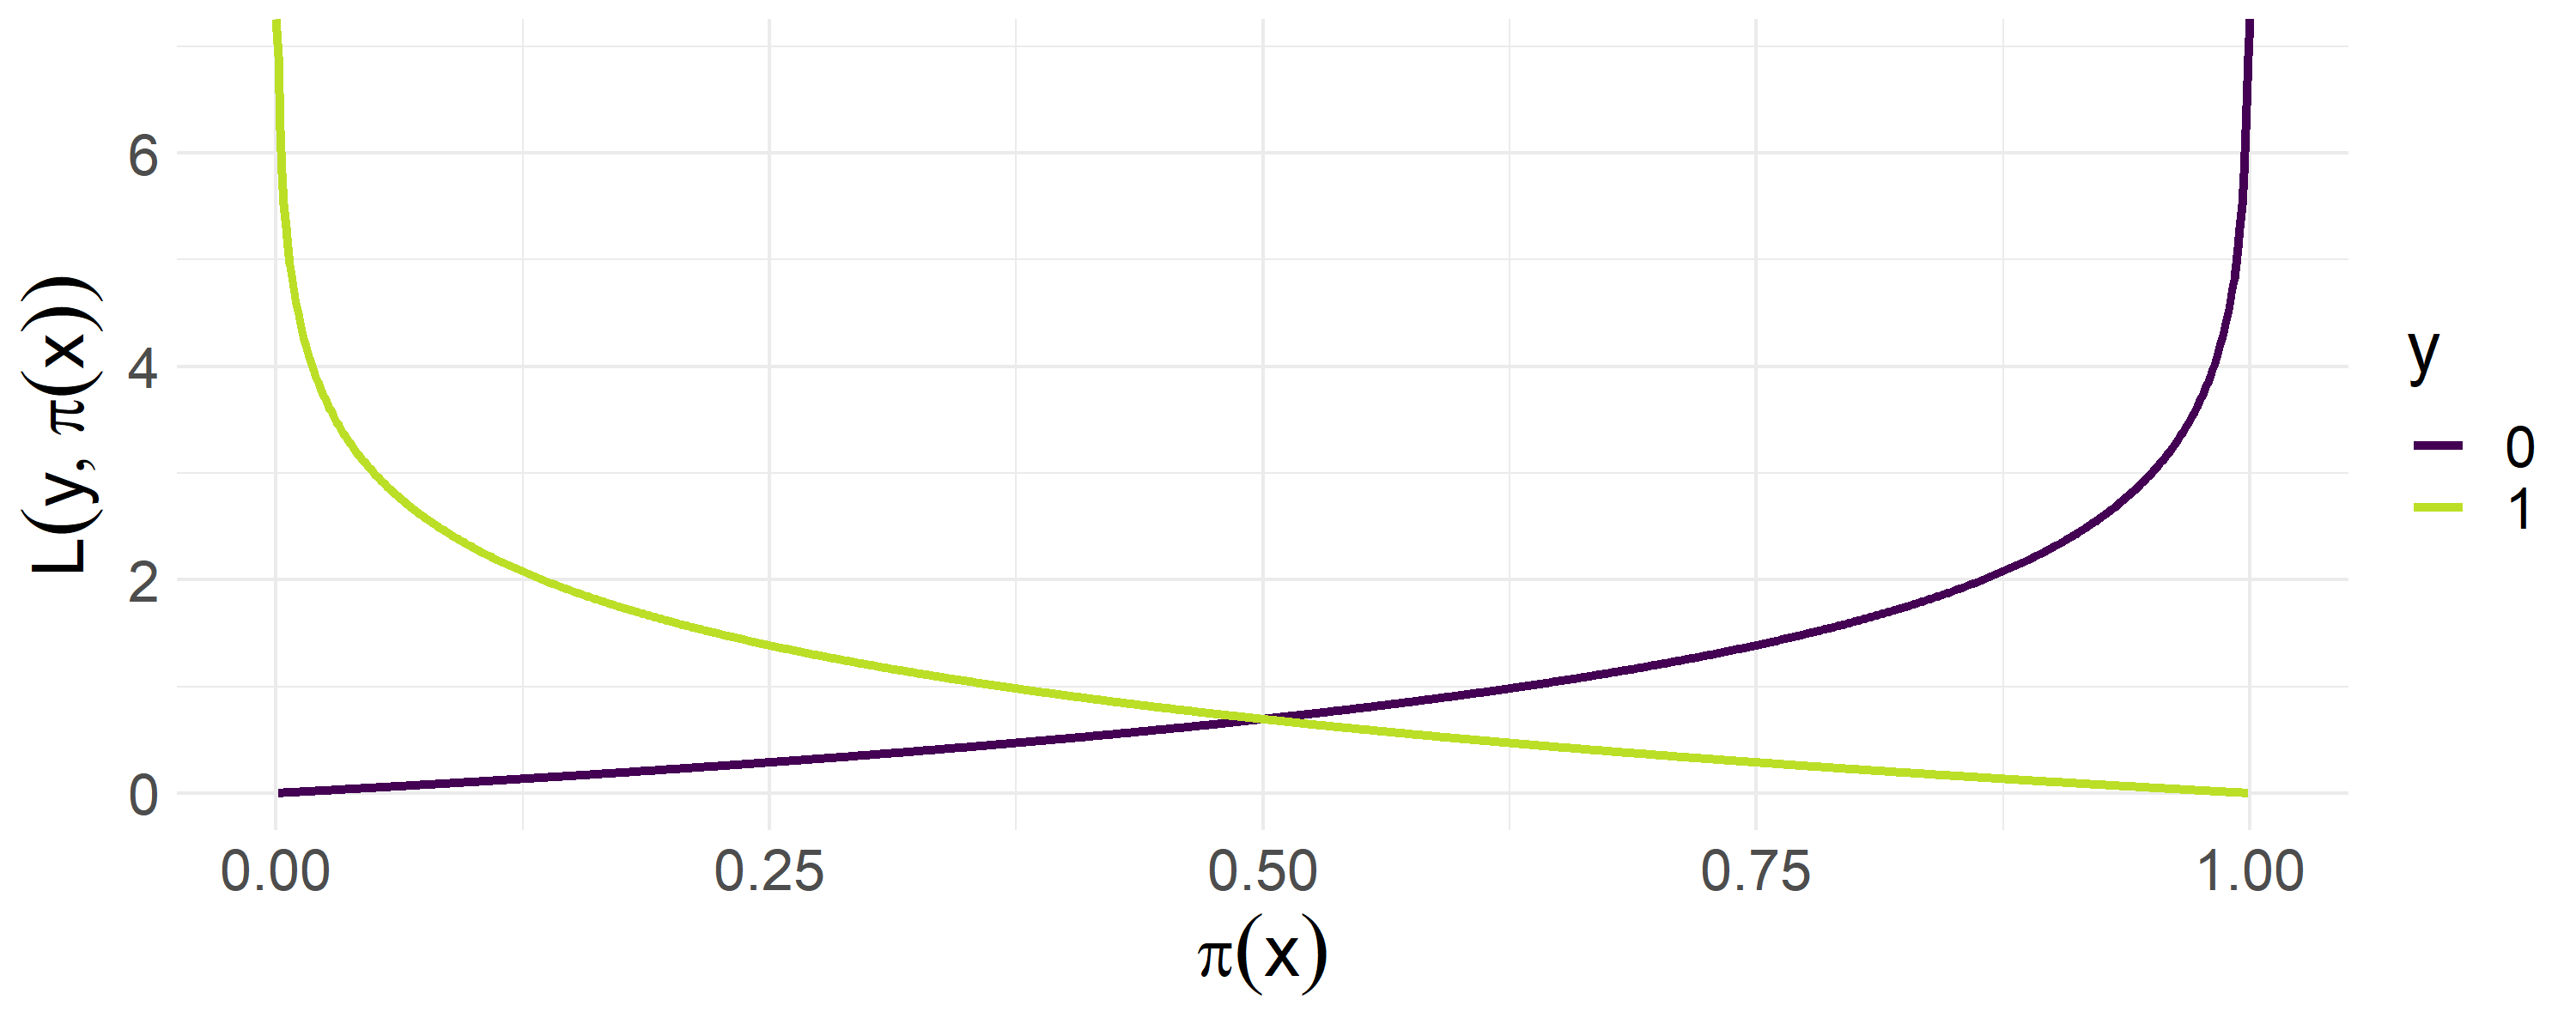
\includegraphics[width = 10cm ]{figure/plot_bernoulli_prob.png}
\end{center}

\end{vbframe}



\begin{vbframe}{Bernoulli loss: Risk Minimizer}

The risk minimizer for the Bernoulli loss defined for probabilistic classifiers $\pix$ and on $y \in \{0, 1\}$ is

$$
  \pixbayes = \eta(\xv) = \P(y = 1 ~|~ \xv = \xv). 
$$

\vspace*{0.2cm}

\begin{footnotesize}
\textbf{Proof:} We can write the risk for binary $y$ as follows: 

% Again, we make use of the law of total expectation

% \begin{eqnarray*}
%   \riskf  & = & \Exy\left[\Lxy\right] = \E_x \left[ \E_{y|x} [ L(y, \fx) ] \right] \\
%           & = & \E_x \left[\sum_{k \in \Yspace} L(k, \fx) \P(y = k~|~ \xv = \xv)\right]\,. 
%           % & = & E_x \sum_{k \in \Yspace} L(k, \fx) \pikx,
% \end{eqnarray*}

% In the binary case this becomes 

% \vspace*{-0.3cm}

\vspace*{-0.3cm}

\begin{eqnarray*}
  \riskf &=& \E_x \left[L(1, \pix) \cdot \eta(\xv) + L(0, \pix) \cdot (1 - \eta(\xv)) \right],
\end{eqnarray*}

with $\eta(\xv) = \P(y = 1 ~|~ \xv)$ (see chapter on the 0-1-loss for more details). 

For a fixed $\xv$ we compute the point-wise optimal value $c$ by setting the derivative to $0$: 

\vspace*{-0.3cm}

\begin{eqnarray*}
  \frac{\partial }{\partial c} \left(- \log c  \cdot \eta(\xv)- \log (1 - c) \cdot (1 - \eta(\xv))\right) &=& 0 \\
  - \frac{\eta(\xv)}{c} + \frac{1 - \eta(\xv)}{1 - c} &=& 0 \\
  % - \frac{\eta(\xv) (1 - c)}{c (1 - c)} + \frac{c(1 - \eta(\xv))}{c(1 - c)} &=& 0 \\
  \frac{- \eta(\xv) + \eta(\xv) c + c - \eta(\xv) c}{c (1 - c)} &=& 0 \\
  c &=& \eta(\xv). 
\end{eqnarray*}

\end{footnotesize}

\framebreak 

The risk minimizer for the Bernoulli loss defined on $y \in \{-1, 1\}$ and scores $\fx$ is the point-wise log-odds:

\begin{eqnarray*}
\fxbayes &=&  \log \biggl(\frac{\P(y~|~\xv = \xv)}{1-\P(y~|~\xv = \xv)}\biggr).
\end{eqnarray*}

The function is undefined when $P(y~|~\xv = \xv) = 1$ or $P(y~|~\xv = \xv) = 0$, but predicts a smooth curve which grows when $P(y~|~\xv = \xv)$ increases and equals $0$ when $P(y~|~\xv = \xv) = 0.5$.

\lz 

\textbf{Proof: } As before we minimize 

\begin{eqnarray*}
  \riskf &=& \E_x \left[L(1, \fx) \cdot \eta(\xv) + L(-1, \fx) \cdot (1 - \eta(\xv)) \right] \\
  &=& \E_x \left[ \log(1 + \exp(- \fx)) \eta(\xv)+ \log(1 + \exp(\fx)) (1 - \eta(\xv)) \right] 
\end{eqnarray*}

\framebreak 

For a fixed $\xv$ we compute the point-wise optimal value $c$ by setting the derivative to $0$: 


\begin{footnotesize}
  \begin{eqnarray*}
  \frac{\partial }{\partial c} \log(1 + \exp(-c)) \eta(\xv)+ \log(1 + \exp(c)) (1 - \eta(\xv)) &=& 0 \\
  - \frac{\exp(-c)}{1 + \exp(-c)} \eta(\xv) + \frac{\exp(c)}{1 + \exp(c)} (1 - \eta(\xv)) &=& 0 \\ 
   - \frac{\exp(-c)}{1 + \exp(-c)} \eta(\xv) + \frac{1}{1 + \exp(- c)} S(1 - \eta(\xv)) &=& 0\\ 
  % &=& -  \frac{\exp(-c)}{1 + \exp(-c)} p + \frac{1}{1 + \exp(-c)} - \frac{1}{1 + \exp(-c)} p \\
  - \eta(\xv) + \frac{1}{1 + \exp(-c)} &=& 0\\
  \eta(\xv) &=& \frac{1}{1 + \exp(-c)} \\
   c &=& \log\left(\frac{\eta(\xv)}{1 - \eta(\xv)}\right)
  \end{eqnarray*}
\end{footnotesize}

\end{vbframe}



\begin{vbframe}{Bernoulli: Optimal constant Model}

The optimal constant probability model $\pix = \theta$ w.r.t. the Bernoulli loss for labels from $\Yspace = \setzo$ is:

\begin{eqnarray*}
  \thetah = \argmin_{\theta} \risket = \frac{1}{n} \sumin \yi
\end{eqnarray*}

Again, this is the fraction of class-1 observations in the observed data.
We can simply prove this again by setting the derivative of the risk to 0 and solving for $\theta$.

\framebreak

The optimal constant score model $\fx = \theta$ w.r.t. the Bernoulli loss labels from $\Yspace = \setmp$ or $\Yspace = \setzo$ is:

\begin{eqnarray*}
  \thetah = \argmin_{\theta} \risket = \log \frac{\np}{\nn} = \log \frac{\np / n}{\nn /n} 
\end{eqnarray*}

where $\nn$ and $\np$ are the numbers of negative and positive observations, respectively.

\lz

This again shows a tight (and unsurprising) connection of this loss to log-odds.

\lz

Proving this is also a (quite simple) exercise.

\end{vbframe}

\begin{vbframe}{Bernoulli-Loss: Naming Convention}

We have seen three loss functions that are closely related. In the literature, there are different names for the losses: 

\begin{eqnarray*}
  L(y, \fx) &=& \log(1+\exp(-y\fx)) \quad \text{for } y \in \setmp \\
  L(y, \fx) &=& - y \cdot \fx + \log(1 + \exp(\fx)) \quad \text{for } y \in \setzo 
\end{eqnarray*}

are referred to as Bernoulli, Binomial or logistic loss. 

  $$
    L(y, \pix) = - y \log \left(\pix\right) - (1 - y) \log \left(1 - \pix\right) \quad \text{for } y \in \setzo
  $$

is referred to as cross-entropy or log-loss. 

\lz 

We usually refer to all of them as \textbf{Bernoulli loss}, and rather make clear whether they are defined on labels $y \in \setzo$ or $y \in \setmp$ and on scores $\fx$ or probabilities $\pix$. 

\end{vbframe}



\begin{vbframe}{Bernoulli loss min = Entropy splitting}

When fitting a tree we minimize the risk within each node $\Np$ by risk minimization and predict the optimal constant. Another approach that is common in literature is to minimize the average node impurity $\text{Imp}(\Np)$. 

\vspace*{0.2cm}

\textbf{Claim:} Entropy splitting $\text{Imp}(\Np) = -\sum_{k = 1}^g \pikN \log \pikN$ is equivalent to minimize risk measured by the Bernoulli loss. 

\begin{footnotesize}
Note that $\pikN := \frac{1}{n_{\Np}} \sum\limits_{(\xv,y) \in \Np} [y = k]$. 
\end{footnotesize}

\vspace*{0.2cm}

\textbf{Proof: } To prove this we show that the risk related to a subset of observations $\Np \subseteq \D$ fulfills 

\vspace*{- 0.2cm}


$$
  \risk(\Np) = n_\Np \text{Imp}(\Np),
$$
  
  where 
  %$I$ is the entropy criterion $\text{Imp}(\Np)$ and 
  $\risk(\Np)$ is calculated w.r.t. the (multiclass) Bernoulli loss  

$$
  L(y, \pix) = -\sum_{k = 1}^g [y = k] \log \left(\pi_k(\xv)\right).
$$

\framebreak 
\begin{footnotesize}
\begin{eqnarray*}
\risk(\Np) &=& \sum_{\xy \in \Np} \left(- \sum_{k = 1}^g [y = k] \log \pi_k(\xv) \right) \\
&\overset{(*)}{=}& -\sum_{k = 1}^g \sum_{\xy \in \Np} [y = k]\log \pikN \\
&=& -\sum_{k = 1}^g \log \pikN \underbrace{\sum_{\xy \in \Np} [y = k]}_{n_{\Np}\cdot \pikN } \\
 &=& -n_{\Np} \sum_{k = 1}^g \pikN \log \pikN = n_\Np \text{Imp}(\Np), 
\end{eqnarray*} 

where in $^{(*)}$ the optimal constant per node $\pikN = \frac{1}{n_{\Np}} \sum\limits_{(\xv,y) \in \Np} [y = k]$ was plugged in. 
\end{footnotesize}
% \framebreak

% \textbf{Conclusion}: 
% \begin{itemize}
%   \item Stumps/trees with entropy splitting use the same loss function as logistic regression (binary) / softmax regression (multiclass).
%   \item    While logistic regression is based on the hypothesis space of \textbf{linear functions}, stumps/trees use \textbf{step functions} as hypothesis spaces. 

% \end{itemize}  

\end{vbframe}







% \vspace*{-0.2cm}

% \begin{eqnarray*}
%   \Lxy = \log \left[1 + \exp \left(-y\fx\right)\right].
% \end{eqnarray*}

% We transform scores into probabilities by

% $$
% \pix = \P(y = 1 ~|~\xv) = s(\fx) = \frac{1}{1 + \exp(- \fx)},
% $$

% with $s(.)$ being the logistic sigmoid function as introduced in chapter 2.

% \framebreak

% As already shown before, an equivalent approach that directly outputs probabilities $\pix$ is minimizing the \textbf{Bernoulli loss}

% \begin{eqnarray*}
% \Lxy = -y \log \left(\pix\right) - (1 - y) \log \left(1 - \pix\right)
% \end{eqnarray*}

% for $\pix$ in the hypothesis space

% \begin{eqnarray*}
%   \Hspace = \left\{\pi: \Xspace \to [0, 1] ~|~\pix = s(\thetab^\top \xv)\right\}
% \end{eqnarray*}

% with $s(.)$ again being the logistic function.

% \framebreak


% Logistic Regression with one feature $\xv \in \R$. The figure shows how $\xv \mapsto \pix$.

% <<fig.height=4>>=
% set.seed(1234)
% n = 20
% x = runif(n, min = 0, max = 7)
% y = x + rnorm(n) > 3.5
% df = data.frame(x = x, y = y)

% model = glm(y ~ x,family = binomial(link = 'logit'), data = df)
% df$score = predict(model)
% df$prob = predict(model, type = "response")
% x = seq(0, 7, by = 0.01)
% dfn = data.frame(x = x)
% dfn$prob = predict(model, newdata = dfn, type = "response")
% dfn$score = predict(model, newdata = dfn)

% p2 = ggplot() + geom_line(data = dfn, aes(x = x, y = prob))
% p2 = p2 + geom_point(data = df, aes(x = x, y = prob, colour = y), size = 2)
% p2 = p2 + xlab("x") + ylab(expression(pi(x)))
% p2 = p2 + theme(legend.position = "none")
% p2
% @

% \framebreak

% Logistic regression with two features:

\endlecture

\end{document}